\chapter{Modélisation}

La modélisation commence à partir des fichiers régionaux produits par le feature engineering. L'objectif est d'entraîner plusieurs familles de modèles afin de prédire la variabilité future de la production solaire normalisée. La démarche est volontairement progressive : partir d'une baseline simple, tester des modèles linéaires interprétables, explorer des modèles plus complexes, puis sélectionner un modèle final selon des critères de performance et de généralisation.

\section{Organisation des ensembles et métriques}

Les jeux de données chargés dans le notebook contiennent les variables régionales finales et la cible \textit{target}. Après séparation entre variables explicatives et cible, les tailles utilisées pour la modélisation sont les suivantes :

\begin{figure}[htbp]
    \centering
    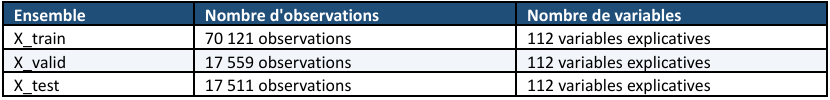
\includegraphics[width=0.8\textwidth]{img/tab_6_1.png}
    \caption{Dimensions des ensembles utilisés après séparation entre X et y.}
    \label{fig:tab_6_1}
\end{figure}

Comme les données sont temporelles, la validation croisée est également construite de manière chronologique. Chaque fold entraîne le modèle sur une période passée et le valide sur une période future. Cette stratégie permet d'évaluer la stabilité temporelle des modèles et d'éviter la fuite d'information.

\begin{figure}[htbp]
    \centering
    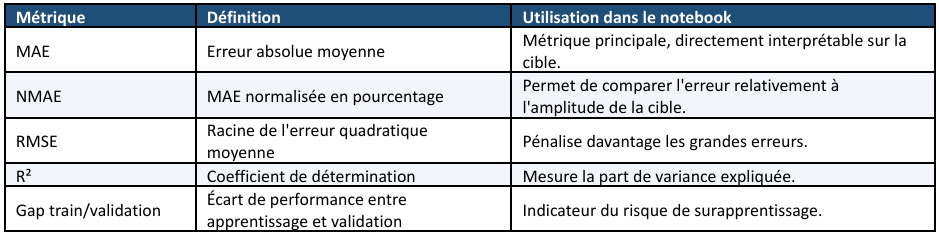
\includegraphics[width=0.9\textwidth]{img/tab_6_2.png}
    \caption{Métriques utilisées pour comparer les modèles.}
    \label{fig:tab_6_2}
\end{figure}

La MAE est privilégiée car elle mesure directement l'erreur moyenne sur l'amplitude de la variabilité prédite. Cependant, la sélection finale ne repose pas uniquement sur la MAE. Le RMSE et le gap entre entraînement et validation sont également considérés pour éviter de retenir un modèle trop optimiste ou trop instable.

\section{Baseline naïve et modèles linéaires}

La première étape consiste à établir un niveau minimal de performance. La baseline naïve prédit que la variabilité future sera proche de la dernière variation absolue observée de la production solaire normalisée, représentée par la variable \textit{dtch\_solaire\_abs\_dt}. Cette référence est importante : un modèle avancé doit faire mieux que cette règle simple pour être réellement utile.

\begin{figure}[htbp]
    \centering
    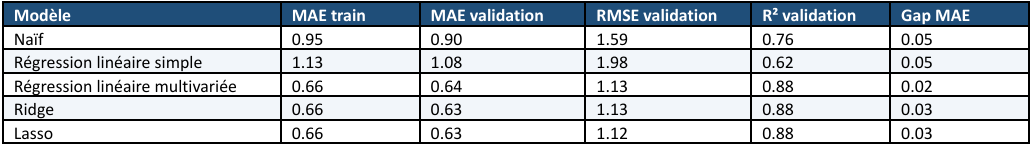
\includegraphics[width=0.9\textwidth]{img/tab_6_3.png}
    \caption{Performances des références naïves et linéaires sur validation.}
    \label{fig:tab_6_3}
\end{figure}

La régression linéaire simple basée uniquement sur la variation de GHI reste inférieure à la baseline naïve. Cela montre que la variabilité de la production ne peut pas être expliquée correctement par une seule variable radiative. Les modèles linéaires multivariés améliorent nettement les performances et atteignent un R² de validation proche de 0,88. Ils constituent donc une référence solide, mais ils restent moins performants que les modèles non linéaires optimisés.

\section{Sélection exploratoire et optimisation des modèles}

Après les modèles linéaires, on utilise le modèle LazyPredict pour obtenir une première comparaison rapide de plusieurs familles de modèles. Cette étape n'est pas utilisée comme évaluation finale, mais elle oriente le choix des modèles à optimiser plus finement. Les modèles d'arbres et de boosting apparaissent comme les plus prometteurs.

\begin{figure}[htbp]
    \centering
    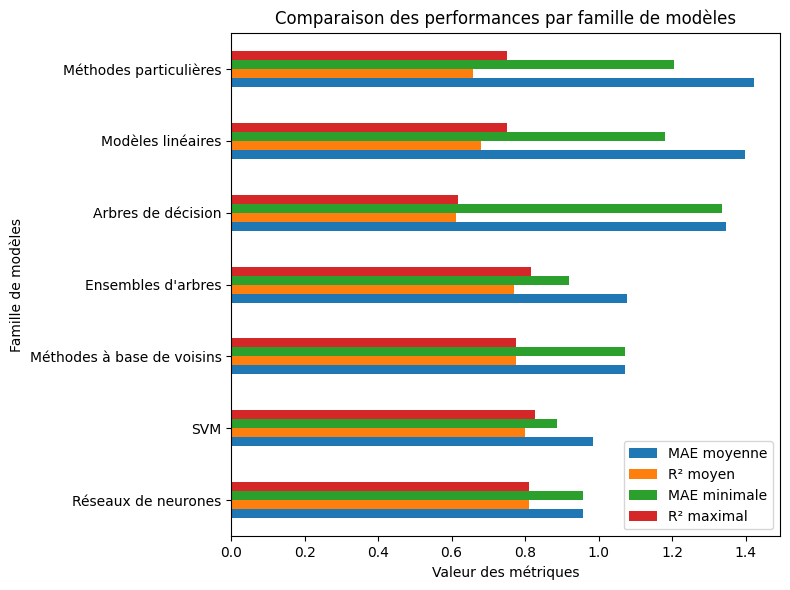
\includegraphics[width=0.8\textwidth]{img/metriques.png}
    \caption{Comparaison exploratoire des performances par famille de modèles.}
    \label{fig:metriques}
\end{figure}

Les modèles retenus pour l'optimisation détaillée comprennent LightGBM, XGBoost, ExtraTreesRegressor, RandomForestRegressor, HistGradientBoostingRegressor et un réseau de neurones MLP. Les hyperparamètres sont optimisés avec Optuna en utilisant les folds temporels définis manuellement. Cette méthode permet de tester de nombreuses combinaisons tout en respectant la structure chronologique des données.

\clearpage

\begin{figure}[htbp]
    \centering
    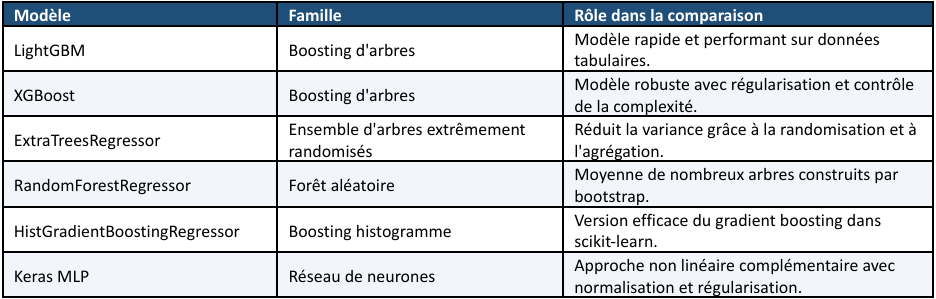
\includegraphics[width=0.9\textwidth]{img/tab_6_4.png}
    \caption{Familles de modèles optimisées dans le notebook.}
    \label{fig:tab_6_4}
\end{figure}

Les visualisations réel/prédit sur validation complètent les métriques numériques. Elles permettent de repérer si les modèles suivent correctement la tendance générale ou s'ils saturent pour les fortes variations. Ces figures montrent globalement une bonne concentration autour de la diagonale, mais aussi une dispersion plus importante pour les valeurs élevées de variabilité, ce qui est fréquent dans les problèmes de rampes solaires.

\begin{figure}[htbp]
    \centering
    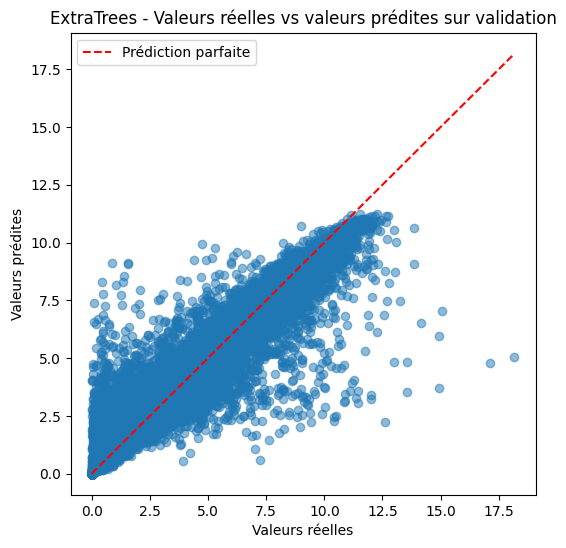
\includegraphics[width=0.5\textwidth]{img/extra_trees.png}
    \caption{ExtraTrees : valeurs réelles et prédites sur l'ensemble de validation.}
    \label{fig:extra_trees}
\end{figure}

\section{Choix du modèle final et évaluation sur test}

Après l'optimisation, les modèles sont comparés à partir d'un score combinant la MAE de validation, le RMSE de validation et le gap de MAE entre entraînement et validation. Ce score est donné par la formule :

\begin{equation}
score = MAE_{valid} + RMSE_{valid} + \frac{Gap_{MAE}}{MAE_{valid}}
\end{equation}

Cette stratégie évite de choisir uniquement le modèle avec la plus petite erreur moyenne si ce modèle présente un comportement moins stable.

\clearpage

\begin{figure}[htbp]
    \centering
    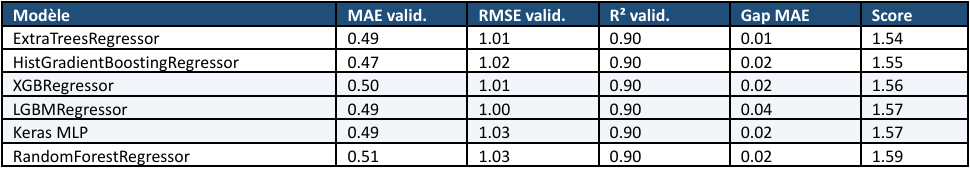
\includegraphics[width=0.9\textwidth]{img/tab_6_5.png}
    \caption{Classement des principaux modèles avant l'évaluation finale sur test.}
    \label{fig:tab_6_5}
\end{figure}

\begin{figure}[htbp]
    \centering
    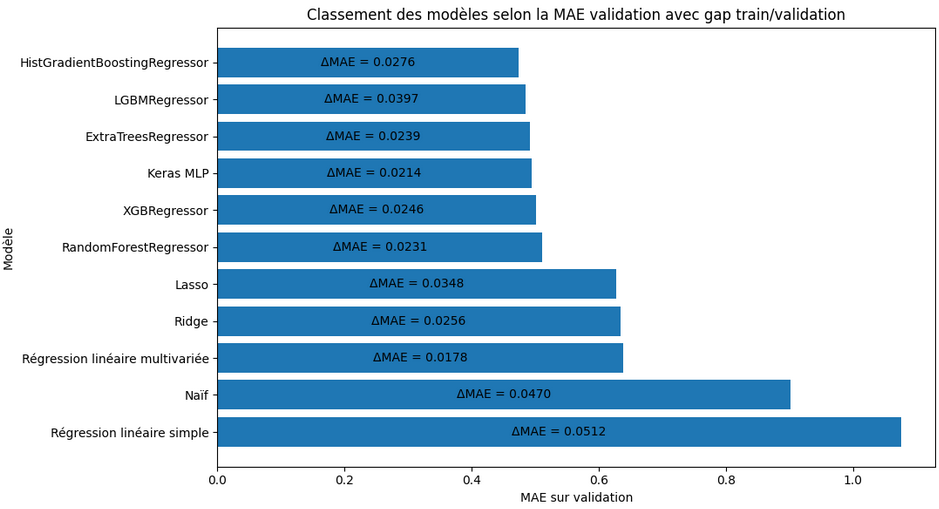
\includegraphics[width=0.9\textwidth]{img/classement.png}
    \caption{Classement des modèles selon le score de validation.}
    \label{fig:classement}
\end{figure}

Le modèle retenu est \textbf{ExtraTreesRegressor}. Il n'est pas seulement performant en validation : il présente aussi un écart train/validation faible et un bon compromis entre MAE, RMSE et R². Une fois ce choix effectué, le modèle est réentraîné sur l'ensemble de développement, c'est-à-dire la réunion de train et validation, puis évalué une seule fois sur le test.

\begin{figure}[htbp]
    \centering
    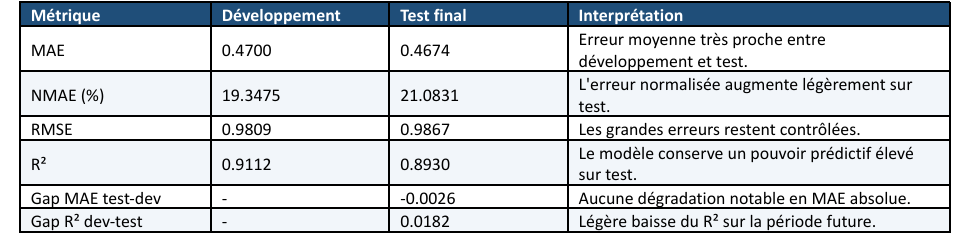
\includegraphics[width=0.9\textwidth]{img/tab_6_6.png}
    \caption{Évaluation finale du modèle ExtraTreesRegressor sur le jeu de test.}
    \label{fig:tab_6_6}
\end{figure}

\clearpage

\begin{figure}[htbp]
    \centering
    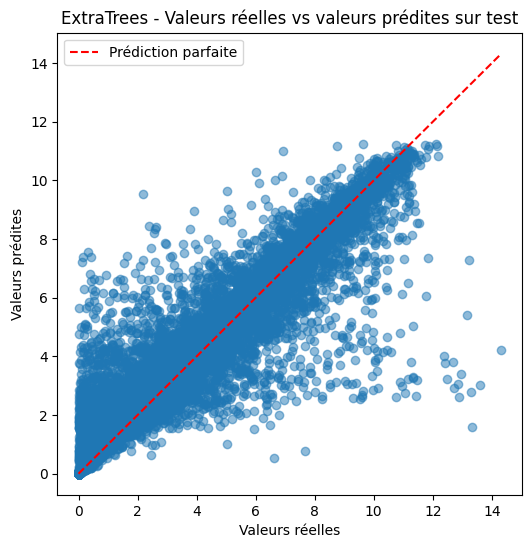
\includegraphics[width=0.5\textwidth]{img/pred_test.png}
    \caption{ExtraTrees : valeurs réelles et prédites sur l'ensemble de test.}
    \label{fig:pred_test}
\end{figure}

Les résultats finaux montrent que le modèle généralise correctement sur la période de test. La MAE est presque identique entre développement et test, tandis que le R² diminue légèrement. Cette baisse peut être liée à une modification de la distribution des données, à des conditions météorologiques différentes ou à une fréquence plus importante de cas extrêmes. Néanmoins, le R² test reste proche de 0,89, ce qui confirme la capacité du modèle à expliquer une part importante de la variabilité future.
